\documentclass{article}

\usepackage{pgf,tikz,pgfplots}
\pgfplotsset{compat=1.15}
\usepackage{mathrsfs}
\usetikzlibrary{arrows}
\usepackage{amsmath,amssymb}
\usepackage{fullpage}
\usepackage{enumerate}
\usepackage{hyperref}
\usepackage{graphicx}
\usepackage{siunitx}
\graphicspath{{../logos/}}


\begin{document}

\setlength{\tabcolsep}{6pt}
\begin{center} \begin{tabular}{cccc}
	
\includegraphics[height=56pt]{SAMF_logo.jpg} &
	
\includegraphics[height=56pt]{SAICA_logo.jpg} &
	
\includegraphics[height=56pt]{OM_Logo_Stacked_Vignette_on_White_RGB.jpg} &
	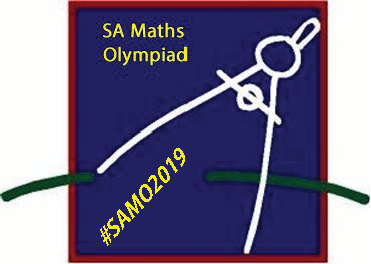
\includegraphics[height=56pt]{SAMO2019.png}
\end{tabular} \end{center}


\bigskip


\begin{center}
	\textbf{\Large Senior Easy Monthly Problem Set :) Solutions}
\end{center}

\begin{enumerate}

\medskip
\item % Emile
{\itshape Pythagoras has discovered pizza! And immediately proceeded to working on combining it with his one true love, rational numbers.

He devises a way to cut a circular pizza such that all cuts go through the center of the pizza and that the ratio of areas of adjacent slices of pizza are rational numbers. He calls such a pizza a \textit{rational} pizza.

Prove that all \textit{rational} pizzas have rational internal angles at the center of the pizza when measured in degrees, as this will make Pythagoras very happy.
}

Suppose the pizza has a radius of $r$. If two adjacent areas have angles $\alpha$ and $\beta$ respectively, then we have that their areas are $\frac{\alpha}{360 \si{\degree}} \times \pi r^2$ and $\frac{\beta}{360 \si{\degree}} \times \pi r^2$ respectively. Thus, the ratio of areas is

$$\frac{\frac{\alpha}{360 \si{\degree}} \times \pi r^2}{\frac{\beta}{360 \si{\degree}} \times \pi r^2} = \frac{\alpha}{\beta} $$

Thus, if the ratio of two areas is rational, the ratio of angles between two consecutive areas must also be rational. If there are $n$ regions with angles $\theta_1$, $\theta_2$, $\cdots$, $\theta_n$. We know that each ratio $\frac{\theta_{i + 1}}{\theta_i}$ is rational. Thus, we must also have that each ratio $\frac{\theta_i}{\theta_1}$ must be rational. Thus, the sum of all the angles is a rational multiple of $\theta_1$. Since the sum of the angles is $360 \si{\degree}$ which is rational, we must have that $\theta_1$ must also be rational and from here we have that all angles must be rational.

\medskip
\item % Emile
{\itshape Define an infinite sequence $a_0$,$a_1$,$a_2$,\ldots by:
\begin{center}
\begin{tabular}{ l l }
    $a_0 = p$ & where $p$ is prime
    \\$a_{n+1} = 2\lfloor \frac{a_n+1}{4}\rfloor + 1$ & if $a_n$ prime, $\forall n \in \mathbb{N}_0$
    \\$a_{n+1} = a_{n} + 1$ & otherwise, $\forall n \in \mathbb{N}_0$
    
\end{tabular}
\end{center}
For which values of $p$ does the series converge?
}


\medskip
\item % Emile
{\itshape Given a triangle, $\triangle ABC$, with $AB = BC$ and circumcenter $O$, let $C'$ be a point on $AB$ such that $AC = AC'$ with $B$ and $C$ on the same side as $A$. Let the circle through $CBC'$ intersect with line $OB$ at $P$, and let $P'$ be the point diametrically opposite $P$. Finally let $Q$ and $Q'$ be the altitudes dropped from $P$ and $P'$ onto $BC$ respectively. Prove $QQ' = BC'$.
}


\medskip
\item % Phil
{\itshape Find all polynomials $P$ with real coefficients such that
\begin{center}
    $P(x^2) + 2P(x) = {P(x)}^2 + 2$
\end{center}
holds for every $x\in\mathbb{R}$
}


\medskip
\item % Ralph
{\itshape Liam and Dylan have been tasked with painting an infinitely long, tiled pavement. Since they would much rather continue their work on solving the Riemann Hypothesis, they have constructed two robots (Liam-bot and Dylan-bot) to do the job for them. Both robots start at the boundary of the first tile. Thereafter, they are only able to walk forward some constant amount, then paint the tile they have landed on, and repeat. If a robot stops on the boundary of two tiles, it paints the tile in front of it. In order to be as efficient as possible, no tile may be painted twice, and every tile must be painted. The first tile is exempted from both of these conditions as Liam and Dylan will paint it themselves. Prove that the distance that Dylan-bot can move in any step is uniquely determined by the distance that Liam-bot can move in any step.
}


\medskip
\item % AoPS
{\itshape 
Given $a$,$b$,$c\in\mathbb{R}$ with $a$,$b$,$c\leq 1$ and $a+b+c = 1$, prove that:
\begin{center}
   $\sum_{cyc} \sqrt{a^2+2b+1}\geq 4$ 
\end{center}
And find when equality occurs.}


\medskip
\item % Korea 2001
{\itshape Given $n$ distinct lattice points $(x_1,y_1),(x_2,y_2),\ldots,(x_n,y_n)$ and given that $|x_iy_{j}-y_ix_{j}| = 1$ if $i-j\equiv_n 1$;
Find all $n$ for where there is guaranteed to be some pair $(i,j)$ such that $|x_iy_{j}-y_ix_{j}| = 1$ and $i-j\not\equiv_n 1$
}


\medskip
\item % Liam
{\itshape Let $p_n$ denote the $n$-th prime number. Define a sequence $\{a_i\}$ by $a_1 = \frac{1}{2}$, and
$$
a_n = 
\begin{cases}
	\frac{1}{p_n} + a_{n - 1} - \frac{a_{n - 1}}{p_n} \quad \text{if } p_n \equiv _4 1 \\
	\frac{p_na_{n - 1} + 1}{p_n + 1} \quad \text{otherwise}
\end{cases}
$$

Find the value of 
$$\lim_{n \to \infty} a_n.$$
}

\end{enumerate}

\end{document}
